\subsubsection{Second-order scheme}
\label{subsec:second-order-energy}
\Cref{fig:second-order-energy} shows monotone energy decay for all
three time steps, with initial energy approximately
$4.295033\times10^{-2}$.
\Cref{tab:second-order-energy} reports the final ratios and balance
diagnostics; the largest normalized balance defect is
$3.71\times10^{-11}$.
The coarsest time step produces slower late-time decay, which is
retained in the plot. Energy dissipation therefore should not be
interpreted as evidence that the temporal error is negligible.
Since the two schemes also use different spatial approximation
orders, these figures are separate stability tests rather than
a controlled comparison of temporal accuracy. The computations
provide numerical evidence of the discrete dissipation mechanism
at the tested step sizes, not a proof for arbitrary step sizes.

\begin{table}[htbp]
\centering
\caption{Second-order unforced energy test: $K=8$, $T=0.5$.}
\label{tab:second-order-energy}
\small
\begin{tabular}{crr}
\toprule
$\dt$ & $E_h(T)/E_h(0)$ & $\max_n\epsilon_{\rm bal}^n$\\
\midrule
$1/16$ & $1.1117\times10^{-4}$ & $3.71\times10^{-11}$\\
$1/32$ & $2.5984\times10^{-5}$ & $7.77\times10^{-13}$\\
$1/64$ & $1.0438\times10^{-5}$ & $2.67\times10^{-13}$\\
\bottomrule
\end{tabular}
\end{table}

\begin{figure}[htbp]
\centering
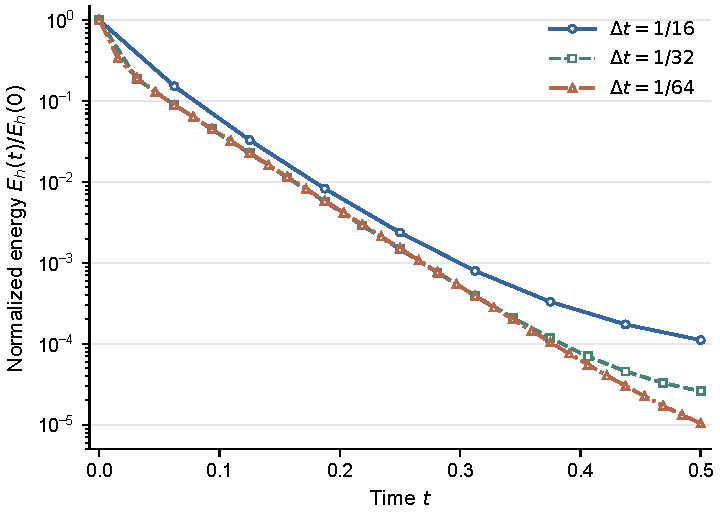
\includegraphics[width=0.70\textwidth]{figures/second_order_energy.pdf}
\caption{Normalized discrete energy for the second-order scheme in the
unforced relaxation test, $K=8$ and $T=0.5$.
The logarithmic vertical scale matches \Cref{fig:first-order-energy}.
Symbols represent all computed time levels without smoothing.
The same discrete initial state is used for all three time steps.}
\label{fig:second-order-energy}
\end{figure}
\FloatBarrier
